% =========================================================================== %
% standalone document to create a scout hello world app
% =========================================================================== %
\documentclass{article}

%=============================================================================%
% Common things, settings, packages to include
%=============================================================================%

\usepackage{graphicx}
\usepackage{color}
\usepackage{makeidx}
\usepackage{ifpdf}
\usepackage{verbatim}

% --------------------------------------------------------------------------- %
% Setting up stuff depeding on output format
% --------------------------------------------------------------------------- %

\ifpdf
  % special settings for pdf mode
  \usepackage[colorlinks]{hyperref}
  \usepackage{courier}
  
  \hypersetup{
    colorlinks,
    linkcolor=darkblue,
    citecolor=darkblue,
    pdftitle={The Eclipse Scout Book},
    pdfauthor={The Scout Community},
    pdfkeywords={Enterprise Framework, Eclipse, Java, Client-Side, Rich Client, Web Client, Mobile},
    pdfsubject={Computer Science}
  }
  
  \usepackage{caption}
  \captionsetup{margin=10pt,font=small,labelfont=bf}
\else
  % special stuff for html mode
  \usepackage[tex4ht]{hyperref}
\fi

% --------------------------------------------------------------------------- %
% Setting up printing range
% --------------------------------------------------------------------------- %

\parindent 1cm
\parskip 0.2cm
\topmargin 0.2cm
\oddsidemargin 1cm
\evensidemargin 0.5cm
\textwidth 15cm
\textheight 21cm

% --------------------------------------------------------------------------- %
% Setting up listings
% --------------------------------------------------------------------------- %

\usepackage{listings}
 
\definecolor{darkviolet}{rgb}{0.5,0,0.4}
\definecolor{darkgreen}{rgb}{0,0.4,0.2} 
\definecolor{darkblue}{rgb}{0.1,0.1,0.9}
\definecolor{darkgrey}{rgb}{0.5,0.5,0.5}
\definecolor{lightblue}{rgb}{0.4,0.4,1}
\definecolor{lightgray}{rgb}{0.97,0.97,0.97}

\renewcommand{\lstlistlistingname}{List of Listings}

% general settings
\lstset{
  basicstyle=\small\ttfamily,
  columns=fullflexible,
  breaklines=true,
  breakindent=10pt,
  prebreak=\mbox{{\color{blue}\tiny$\searrow$}},
  postbreak=\mbox{{\color{blue}\tiny$\rightarrow$}},
  showstringspaces=false,
  backgroundcolor=\color{lightgray}
}

% settings for xml files
\lstdefinelanguage{xml}
{
  commentstyle=\color{darkgrey}\upshape,
  morestring=[b]",
  morestring=[s]{>}{<},
  morecomment=[s]{<?}{?>},
  stringstyle=\color{black},
  identifierstyle=\color{darkblue},
  keywordstyle=\color{cyan},
  morekeywords={xmlns,name,point,factory,class}% list your attributes here
}

% settings for ini files
\lstdefinelanguage{ini}
{
  morecomment=[f][\color{darkgrey}\upshape][0]\#, % # is comment iff it's the first char on the line
  stringstyle=\color{black}
}

% default settings (for java files)
\lstset{
  language=Java,
  emphstyle=\color{red}\bfseries,
  keywordstyle=\color{darkviolet}\bfseries,
  commentstyle=\color{darkgreen},
  morecomment=[s][\color{lightblue}]{/**}{*/},
  stringstyle=\color{darkblue},
}

% --------------------------------------------------------------------------- %
% cross reference macros
% --------------------------------------------------------------------------- %
\newcommand{\applabel}[1]{\label{apx:#1}}
\newcommand{\chalabel}[1]{\label{cha:#1}}
\newcommand{\seclabel}[1]{\label{sec:#1}}
\newcommand{\lstlabel}[1]{\label{lst:#1}}
\newcommand{\figlabel}[1]{\label{fig:#1}}
\newcommand{\tablabel}[1]{\label{tab:#1}}

\newcommand{\appref}[1]{Appendix~\ref{apx:#1}}
\newcommand{\charef}[1]{Chapter~\ref{cha:#1}\xspace}
\newcommand{\secref}[1]{Section~\ref{sec:#1}}
\newcommand{\lstref}[1]{Listing~\ref{lst:#1}\xspace}
\newcommand{\figref}[1]{Figure~\ref{fig:#1}\xspace}
\newcommand{\tabref}[1]{Table~\ref{tab:#1}\xspace}

% --------------------------------------------------------------------------- %
% graphics paths
% --------------------------------------------------------------------------- %
\graphicspath{
  {figures/}
  {Introduction/figures/}
}

%=============================================================================%

\graphicspath{{modules/figures/}}

\begin{document}

% --------------------------------------------------------------------------- %
\section*{The Scout ''Hello World!''}

After installing the Eclipse Scout package you are now ready to implement your first Scout application. 

% --------------------------------------------------------------------------- %
\section*{Create a Scout Project}
% =========================================================================== %
% TeX input file: "Create a new project"
%
% WARNING: this tex file does not compile standalone, it needs to be embedded
% in a master tex document (e.g. Introduction.tex)
% =========================================================================== %

Start your Eclipse IDE and select an empty directory for your workspace. 
This workspace directory will then hold all the project code for the ''Hello World'' application. 
Once the Eclipse IDE is running it will show the Scout perspective with the ''Scout Explorer'' view and an empty ''Scout Object Properties'' view.
To create a new Scout project select the \contextmenu{New Scout Project...} as shown in \figref{sdk_create_new_scout_project}.

\begin{figure}
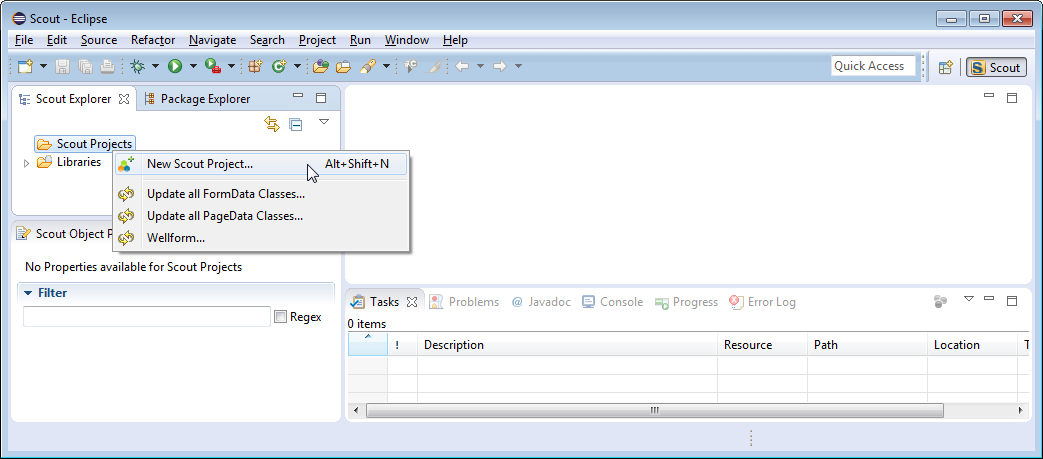
\includegraphics[width=15cm]{sdk_create_new_scout_project.png}
\caption{Create a new Scout project using the Scout SDK perspective.}
\figlabel{sdk_create_new_scout_project}
\end{figure}

In the \wizard{New Scout Project} enter a name for your Scout project. 
As we are creating a ''Hello World'' application, use \java{org.eclipsescout.helloworld} for the \field{Project Name} according to \figref{sdk_new_project_wizard}.
Then, click the \button{Finish} to let the Scout SDK create the initial project code for you.

\begin{figure}
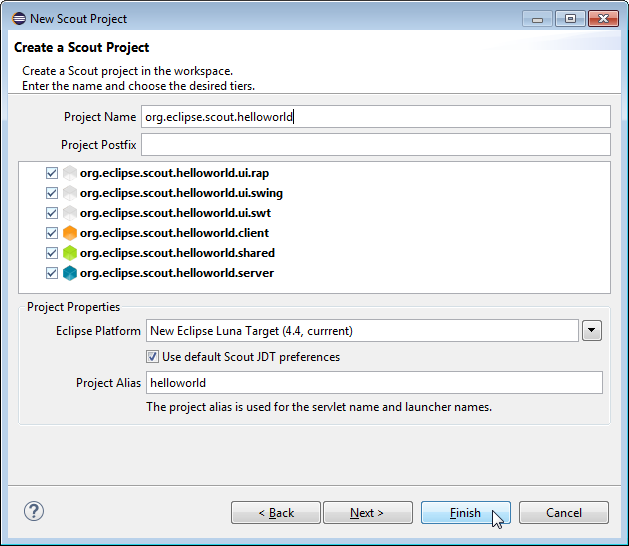
\includegraphics[width=6cm]{sdk_new_project_2.png}
\caption{The new Scout project wizard.}
\index{SDK Wizard!New Scout Project}
\figlabel{sdk_new_project_wizard}
\end{figure}

Once the initial project code is built, the Scout SDK displays the application model in the \textit{Scout Explorer} as shown in \figref{sdk_initial_helloworld_project}.
This model is visually presented as a tree structure covering both the client and the server part of the application.
The Scout Explorer view on the left hand side displays the top level elements of the complete Scout application.
Under the orange node the Scout client components are listed. 
Components that are needed in both the Scout client and the Scout server are collected under the green node.
And the Scout server components are listed below the blue node in the Scout Explorer view.

\begin{figure}
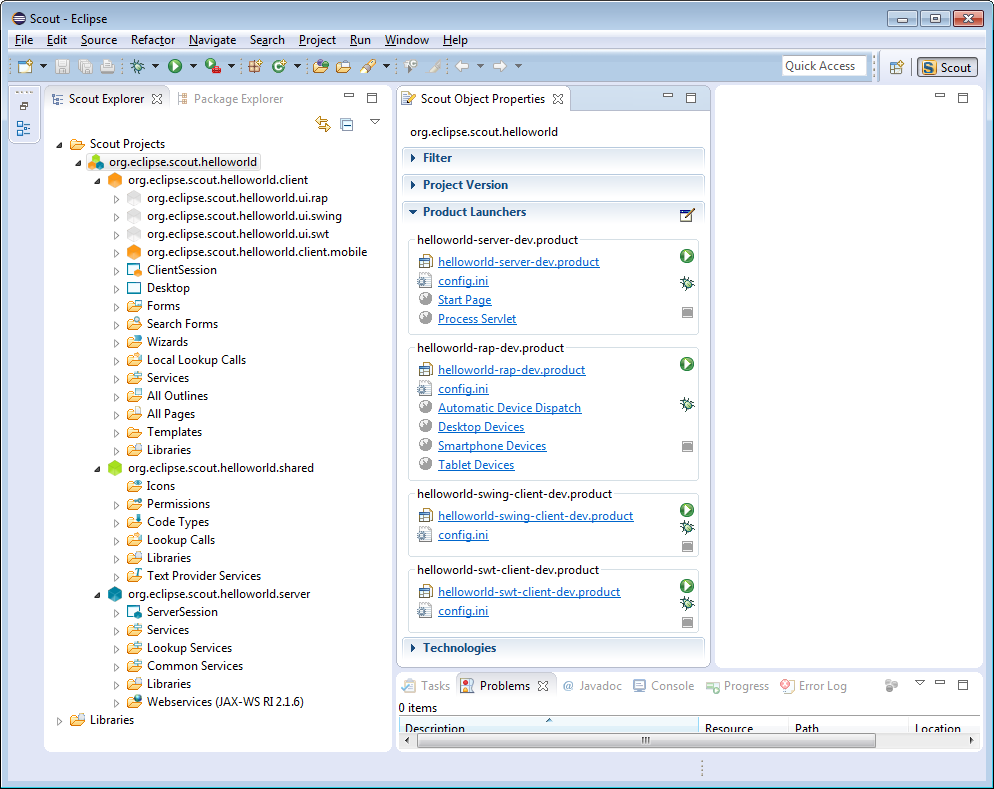
\includegraphics[width=15cm]{sdk_initial_helloworld_project.png}
\caption{The Scout SDK showing the tree representation of our ''Hello World'' application in the Scout Explorer.
The Scout Object Properties contain the product launchers for the server and the available clients.}
\figlabel{sdk_initial_helloworld_project}
\end{figure}

% =========================================================================== %
% EOF TeX input file
% =========================================================================== %

% --------------------------------------------------------------------------- %
\section*{Run the Application}
% =========================================================================== %
% TeX input file: "Run the hello world application"
%
% WARNING: this tex file does not compile standalone, it needs to be embedded
% in a master tex document (e.g. Introduction.tex)
% =========================================================================== %

After the initial project creation step we can start the Scout application for the first time.
For this, we switch to the Scout Explorer view and select the root node \java{org.eclipse.scout.helloworld}.
This then loads the corresponding controls and the \textit{Product Launchers section} into the \textit{Scout Object Properties} view as shown in \figref{sdk_initial_helloworld_project}.

\begin{figure}
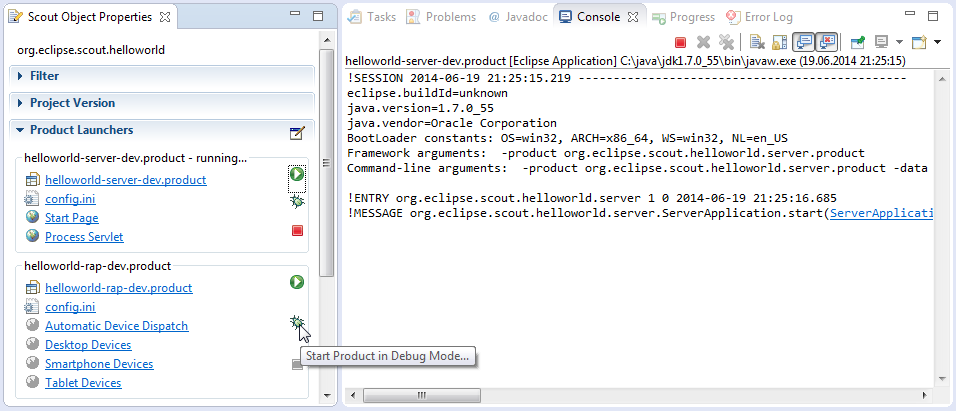
\includegraphics[width=15cm]{sdk_start_client_product.png} 
\caption{Starting the Hello World application in the Scout SDK using the provided product launcher. Make sure to start the server before starting any client product.}
\figlabel{start_client}
\index{Product launchers}
\end{figure}

In the product launcher section of the Scout Object Properties view four launcher boxes are available. 
One launcher box for the Scout server product, and three launchers for the different client products.
Each launcher box provides a link to the corresponding configuration and product definition files, as well as the launcher icons to start and stop the corresponding product.
The green \icon{Circle} starts the product in normal mode.
The \icon{Bug} just below, starts a product in debug mode.
To terminate a running product, the red \icon{Square} is provided. 

Before any of the client products is started, we need to start the server product using the green circle or the bug launcher icon.
During startup of the Scout server you should see console output similar to the one shown on the right hand side of \figref{start_client}.

Once the server is running, you may start the RAP client as shown in \figref{start_client}.
To start the Swing client, or the SWT client use the corresponding green \icon{Circle} or \icon{Bug}.
And with a running RAP client, the Scout client can be opened in a web browser by clicking on the provided \link{Automatic Device Dispatch}.

\begin{figure}
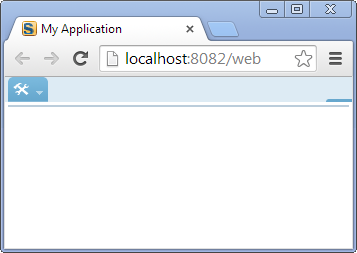
\includegraphics[width=4.5cm]{hellworld_empty_rap.png} \hspace{3mm}
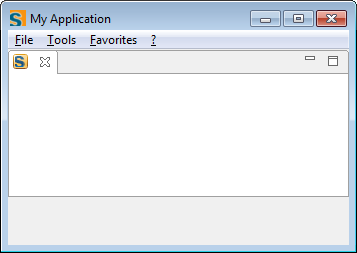
\includegraphics[width=4.5cm]{hellworld_empty_swing.png} \hspace{3mm}
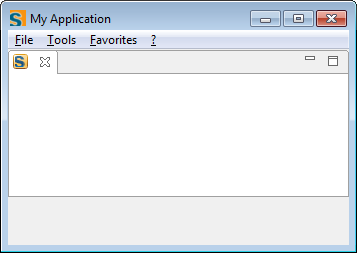
\includegraphics[width=4.5cm]{hellworld_empty_swt.png}
\caption{Running the three client applications. 
Each client displays an empty desktop form. 
The RAP client, the Swing client, and the SWT client}
\figlabel{helloworld_empty}
\end{figure}

Having started the Scout server and all client products, the running client applications should look as shown in \figref{helloworld_empty}.

% =========================================================================== %
% EOF TeX input file
% =========================================================================== %

% --------------------------------------------------------------------------- %
\section*{Add the User Interface Widgets}
% =========================================================================== %
% TeX input file: "Create the hello world frontend"
%
% WARNING: this tex file does not compile standalone, it needs to be embedded
% in a master tex document (e.g. Introduction.tex)
% =========================================================================== %

The project creation step has created a Scout client that displays an empty desktop form.
We will now add widgets to the client's desktop form that will later display the ''Hello World!'' message.

To add any widgets to the desktop form, we first need to navigate to the \element{DesktopForm} in the Scout Explorer.
For this, first navigate to the orange client node in the Scout Explorer view.
Then, expand the \element{Forms} folder by clicking on the small triangle icon, and further expand the \element{DesktopForm}. 
As a result, the \element{MainBox} element becomes visible below the desktop form as shown in \figref{new_field_context_menu}. 
With a click of the right mouse button over the \element{MainBox}, the available context menus are displayed.
To start the form field wizard we select the \menu{New Form Field ...}.

\begin{figure}
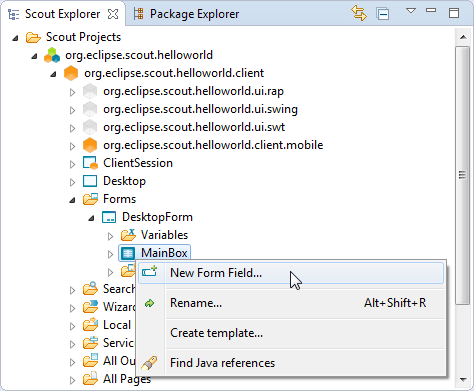
\includegraphics[width=8cm]{sdk_new_field_wizard_menu.png} 
\caption{Using the \menu{New Form Field ...} to start the form field wizard provided by the Scout SDK.}
\figlabel{new_field_context_menu}
\end{figure}

In the first step of the form field wizard shown on in \figref{helloworld_groupboxfield} we choose \java{GroupBox} as the form field type and click on the \button{Next}.
In the second wizard step, we enter 'Desktop' into the \field{Class Name} before we close the wizard with the \button{Finish}.
The Scout SDK will then add the necessary Java code for the \java{DesktopBox} in the background.

\begin{figure}
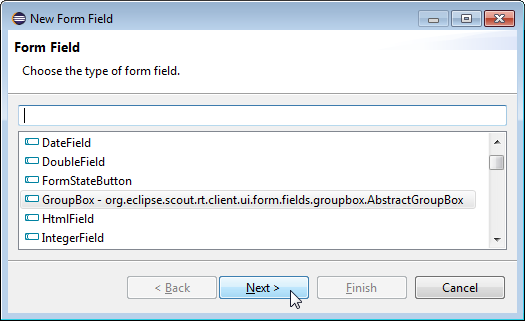
\includegraphics[height=4.5cm]{sdk_new_field_groupbox_1.png} \hspace{8mm}
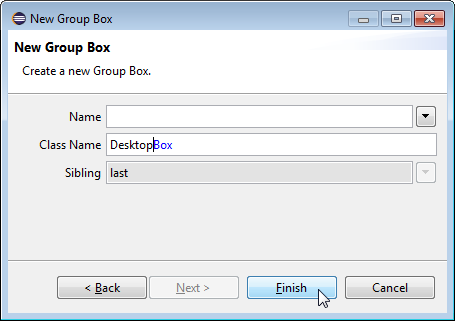
\includegraphics[height=4.5cm]{sdk_new_field_groupbox_2.png}
\caption{Adding the \textit{DesktopBox} field with the Scout SDK form field wizard.}
\index{SDK Wizard!New Form Field}
\figlabel{helloworld_groupboxfield}
\end{figure}

We can now add the text field widget to the group box just created.
To do this, we expand the \element{MainBox} in the Scout Explorer view to access the newly created \element{DesktopBox} element. 
On the \element{DesktopBox} we can then use the \menu{New Form Field ...} again.
In the first wizard step, we select \element{StringField} as the form field type. 
To select the \element{StringField} type you can either scroll down the list of available types or enter ''st'' into the field above the field type list. 

In the second wizard step, we enter 'Message' into the \field{Label}.
As we do not yet have the text 'Message' available in our ''Hello World'' application the wizard prompts the user with the proposal \textsc{New Translated Text ...}.
With a double click on this option a new text entry can be added to the application as shown in \figref{helloworld_stringfield}.
Once we have provided some initial translation for our message label, we can close the translation dialog with the \button{Ok}.
Finally, we close the form field wizard using the \button{Finish}.

\begin{figure}
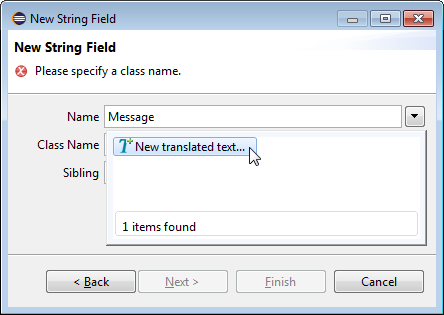
\includegraphics[height=4.2cm]{sdk_new_field_stringfield_1.png} \hspace{8mm}
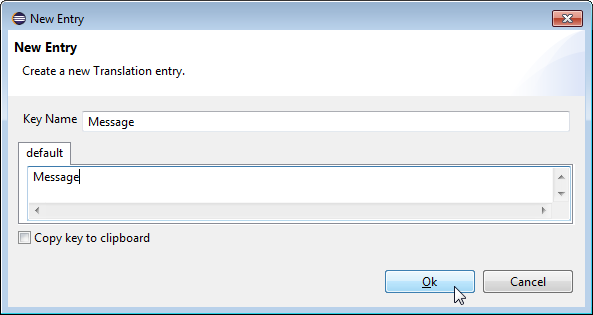
\includegraphics[height=4.2cm]{sdk_new_field_stringfield_2.png}
\caption{Adding a \textit{StringField} and providing a new translation entry.}
\index{SDK Wizard!Add Translation Entry}
\figlabel{helloworld_stringfield}
\end{figure}

By expanding the \element{DesktopBox} element in the Scout Explorer, the new message field becomes visible. 
A double click on the message field element then loads the corresponding Java code into an Editor and displays the message field's properties in the Scout Object Properties as shown in \figref{helloworld_messagefield}.
This is a good moment to compare your status with this screenshot.
Make sure that both the Java code and the project structure in the Scout Explorer look as shown in \figref{helloworld_messagefield}. 

\begin{figure}
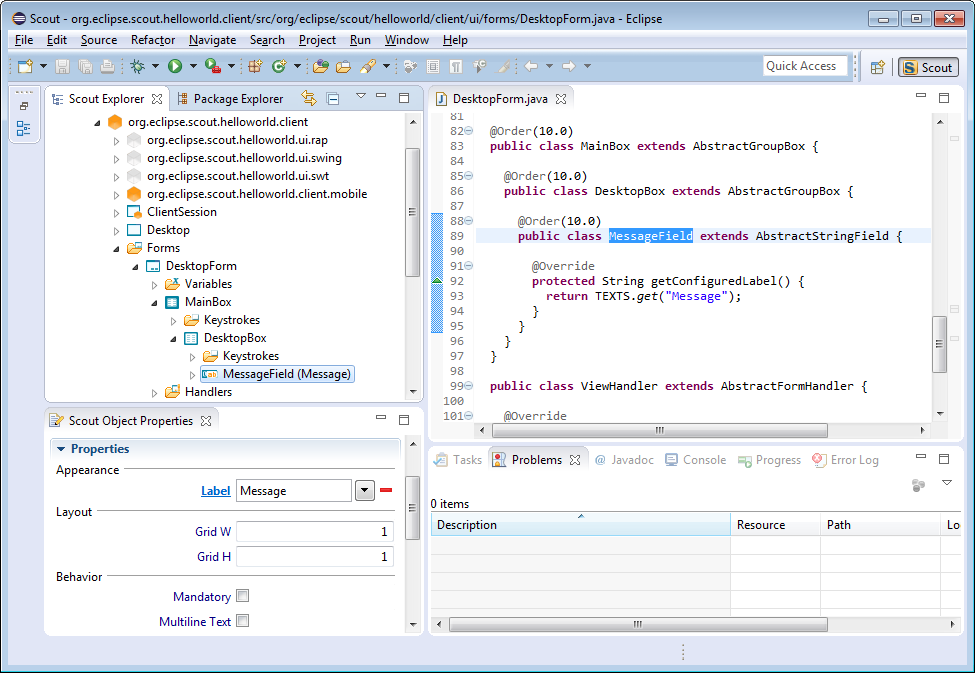
\includegraphics[width=15cm]{sdk_helloworld_messagefield.png}
\caption{Scout SDK showing the \it{MessageField}}
\figlabel{helloworld_messagefield}
\end{figure}

Having verified your status of the ''Hello World'' application you can start the application as described in the previous section.
The client applications will then display your message widget.
However, the text widget is still empty, as we did not yet load any initial content into it.
This is the topic of the next section where we continue this tutorial with the server part.

% =========================================================================== %
% EOF TeX input file
% =========================================================================== %

% --------------------------------------------------------------------------- %
\section*{Implement the Server Service}
% =========================================================================== %
% TeX input file: "Create the hello world backend"
%
% WARNING: this tex file does not compile standalone, it needs to be embedded
% in a master tex document (e.g. Introduction.tex)
% =========================================================================== %

The responsibility of the Scout server in our ''Hello World'' application is to provide an initial text content for the message field in the client's user interface.
We implement this behaviour in the \java{load} method of the server's \java{DesktopService}.
An empty stub for the \java{load} method of the \java{DesktopService} service has already been created during the initial project creation step. 

To navigate to the implementation of the desktop service in the Scout SDK, we first expand the blue top-level \node{server} in the Scout Explorer.
Below the server node, we then expand the \folder{Services} which shows the \element{DesktopService} element.
Expanding this \element{DesktopService} node, the \java{load} method becomes visible as shown in \figref{helloworld_load_servicemethod}.

\begin{figure}
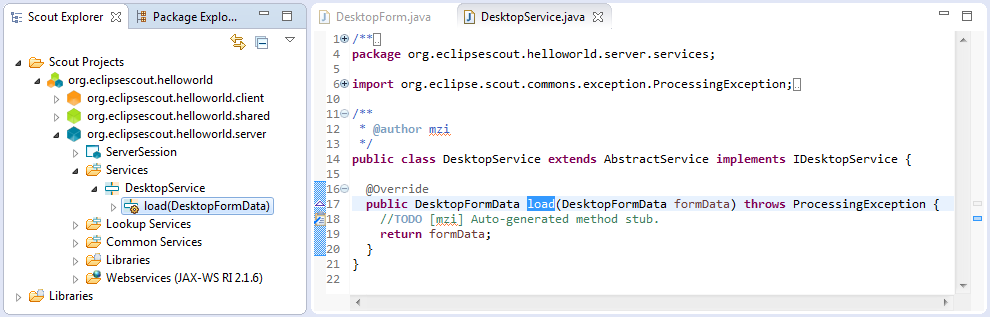
\includegraphics[width=14cm]{sdk_server_desktopservice_load.png}
\caption{The Scout Explorer showing the blue server node expanded with the \folder{Services}.
In this folder the \element{load} method of \element{DesktopService} is selected and its initial implementation is shown in the editor on the right side.}
\figlabel{helloworld_load_servicemethod}
\end{figure}

The \java{DesktopService} represents the server service corresponding to the \java{DesktopForm} on the client side.
This initial setup represents Scout's default where client forms and server services typically come in pairs.
Whenever the client's user interface displays a form to the user, the client connects to the server and calls the \java{load} method of the corresponding server service.
We just need to add our business logic to the \java{load} method of the server's \java{DesktopService}.

According to the signature of the \java{load} method, a \java{formData} object is passed into this method that is then handed back in the return statement.
To complete the implementation of the \java{load} method it is sufficient to assign the text 'hello world!' to the message field part of the form data according to the following line.

\begin{lstlisting}[backgroundcolor=\color{white}]
// test comment
formData.getMessage().setValue("Hello World!");
\end{lstlisting}

The complete implementation of the load method is provided below.
With this last element we have completed the Scout ''Hello World'' application.

\begin{lstlisting}
@Override
public DesktopFormData load(DesktopFormData formData) 
    throws ProcessingException 
{
    formData.getMessage().setValue("Hello World!"); 
    return formData;
}
\end{lstlisting}

% =========================================================================== %
% EOF TeX input file
% =========================================================================== %


% --------------------------------------------------------------------------- %
\section*{Run the Final Application}

We are now ready to run the completed ''Hello World!'' application by first starting the server and then the clients. 
This results in running clients as shown in \figref{helloworld_finished}. 
The mobile version of the client can be started from the Scout SDK by clicking on the \link{Smartphone Devices} in the product launchers section. 
Alternatively, manually change the applications URL from \java{http://localhost:8082/web} to \java{http://localhost:8082/mobile}. 

\begin{figure}
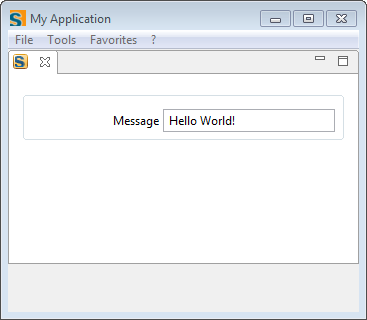
\includegraphics[width=4.5cm]{helloworld_swt.png} \hspace{3mm}
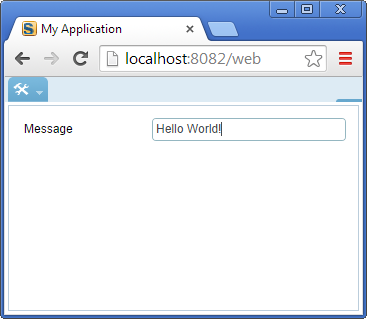
\includegraphics[width=4.5cm]{helloworld_web.png} \hspace{3mm}
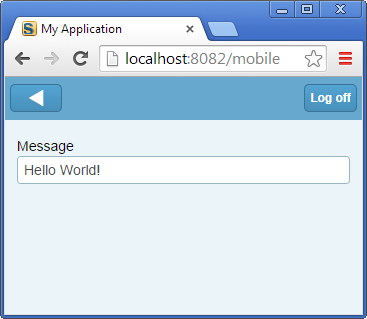
\includegraphics[width=4.5cm]{helloworld_mobile.png}
\caption{Running the complete ''Hello World!'' application with an SWT client, as a web application and a mobile application.}
\figlabel{helloworld_finished}
\end{figure}

Congratulations, you just have implemented your first Scout client server application!

% --------------------------------------------------------------------------- %
\section*{What Next?}

Now that you have successfully created your first Scout application, you might want to learn more about Scout. 
To gain experience with Scout, you can follow more tutorials and start to read in the Scout books.
If you prefer ''Learning by doing'' browse the available Wiki tutorials and go for the subset that matches your interests.

\url{http://wiki.eclipse.org/Scout/Tutorial}

If you are interested in Scout's concepts, architecture and features you probably want to start reading. 
For this, we are writing the Scout books. 

\url{http://wiki.eclipse.org/Scout/Book}

In case you should get stuck somewhere and need help, try to get answers by searching the web. 
And if despite reasonable efforts this approach does not help, contact us on the forum. 
Should you have solved issues on your own, please consider sharing your findings in the Scout forum as this can help other folks too. 

\url{http://www.eclipse.org/forums/eclipse.scout}

We wish you all the best on your journey with Scout and hope to hear from you in the Scout forum.

\end{document}
% =========================================================================== %
